\tbd{rephrase in terms of localization along two dimensions: time, and
component}
In this section we present two mechanisms to facilitate the troubleshooting
process. Correspondence checking allows troubleshooters to isolate
the cause of policy-violations to a particular layer. \Simulator{}
allows troubleshooters to isolate relevant events throughout the system
execution. We provide the details of these techniques below. 

\tbd{define terms early on: event sequence, policy-violation, minimal causal set}

\subsection{Correspondence Checking}

Platform correctness can be expressed as a simple invariant:
the policy specified by the application layer should correspond to the
configuration of the
physical network. We check this invariant by applying the virtual packet
algebra pioneered in headerspace analysis~\cite{hsa}. 

Formally, each layer of the SDN stack can be represented as a graph,
$G = (V, E)$. Packets are series of bits, $h \in \{0,1\}^L = H$,
where $L$ is the maximum number of bits in the header. Upon receiving a packet,
forwarding elements apply a transformation function, potentially modifying
packets before forwarding them on\footnote{Multicast forwarding can expressed
by extending the range to sets of output tuples}:
\begin{align*}
T: (H \times E) \rightarrow (H \times E_{\emptyset})
\end{align*}

We use $`\Psi`$ to denote the collection of all transfer functions present in
the network at a particular point in time. In this model, network traversal is simply a composition of transformation
functions. For example, if a header $h$ enters the network through edge
$e$, its state after $k$ hops will be:
\begin{align*}
\Psi^k(h,e) = \Psi(\Psi(\dots \Psi(h,e)\dots))
\end{align*}

The externally visible behavior of the network can be expressed as the
transitive closure of $\Psi$:
\begin{align*}
\Omega: (H \times E_{access}) \rightarrow (H \times E_{\emptyset}) \\
\Omega(h,e) = \Psi^{\infty}(h,e)
\end{align*}
Here, $E_{access}$ denotes access links adjacent to end-hosts.

In SDN, it should always be the case that:
\begin{align*}
\Omega^{view} \sim \Omega^{physical}
\end{align*}
Informally, this means that any packet injected at an access link in $G^{virtual}$ should arrive at
the same final location as the corresponding (encapsulated) packet injected at the
corresponding access link in $G^{physical}$. Note that hosts are represented
in all graphs, although there may not be a one-to-one mapping between the
internal vertices of $G^{virtual}$ and $G^{physical}$.

To check correspondence in SDN, we begin by taking a causally consistent
snapshot~\cite{Chandy:1985:DSD:214451.214456} of the physical network. The routing
tables of forwarding elements can then be translated into transformation functions.
Finally, we feed a symbolic packet $x^L$ to each access link of the
network.\footnote{The rules for process wildcard bits $x^n$ are defined in
the HSA paper~\cite{hsa}} The end result is a propagation graph representing all possible paths taken by a packet injected
at the access link.

The leaves of the propagation graph represent $\Omega$. We
verify correspondence in SDN by generating propagation graphs for all SDN layers,
and comparing the leaves. Any mismatch in leaves of the propagation graphs
represent policy-violations between control applications and network
configuration.

\subsection{\SIMULATOR{}}

\colin{Insight: policy-violations are unavoidable in distributed systems
(delay). $\rightarrow$ Challenge is to distinguish pernicious from benign
policy-violations}

\begin{itemize}
\item Motivate with a (real?) example
\item Normal software practices -> regression tests: collect failure modes
\item Large failure log
\item failure events numerous, potentially overlapping, unclear which are important
\item We offer an improvement: track policy-violation over time to find “minimal
\item causal set”
\item Takeaway: “I have never seen this in a networked system”
\end{itemize}

\colin{Step backwards, not forwards}

Correspondence checking only captures a snapshot of the network state.
We have developed \simulator{} to allow enable troubleshooters to explore
policy-violations over time. We base our replay on a consistent
trace of low level failure and topology change events, as enabled,
\eg{}, by OFRewind~\cite{ofrewind}. The
events from the trace are fed into a simulator, which allows the
troubleshooter to invokes correspondence
checking at any point in time. The simulator focuses on corner-case events,
and models the failure modes in sufficient detail to reproduce the error, while
allowing for complete control of the timing, ordering, and construction of the events.

%and does not enable the troubleshooter to classify the
%gravity of the detected inconsistencies, i.e., whether the detected 
%inconsistencies are temporary, i.e., byproducts of the forwarding reconverging 
%after a link failure, or whether they are and persistent.
%Also, it cannot aid in isolating the precise \emph{even sequence} that triggered
%the faulty behavior.

If users were to run \simulator{} on raw event logs, they would encounter a
large number of failure events and transient policy-violations. We describe
how users can apply \simulator{} to differentiate transient from persistent
policy-violations below.

\textbf{Identifying persistent policy-violations}. When a policy-violation is detected,
the simulators forks off a simulation branch that investigates the future system behavior
in a case where no further external events are played out. If the detected
policy-violation
is resolved in isolation within a customizable number of simulation time steps, it is considered
a temporary problem. If it is not, this is a strong indication that the system has indeed
reached a persistent policy-violation that needs to be investigated.

\textbf{Checking related problems by fuzzing.} Input traces can be \emph{fuzzed}, i.e.,
randomly perturbed, to expose the system to similar error conditions, and confirm
that a proposed solution is not just a point-fix.

\textbf{Investigating pathological environment conditions.} The simulator allows for investigation
of pathological environment conditions difficult to achieve in a real world test bed
(\eg{}, correlated failure rates, extremely long delays etc.). This enables
investigation of situations that have a high potential for triggering errors.

\textbf{Interactive exploration.} Troubleshooters can also interactively bisect
the trace or modify specific events to further pinpoint the cause for a failure.
This is useful as soon as a suspect event sequence has been identified.

\textbf{regression/integration test.} Library of known tricky scenarios.
\colin{Way to frame this: the value of a regression library may seem obvious to you
systems researchers, but it's new to us networks researchers :). We've never
seen this before in a networked system!}

\begin{figure}[t]
    %\hspace{-10pt}
    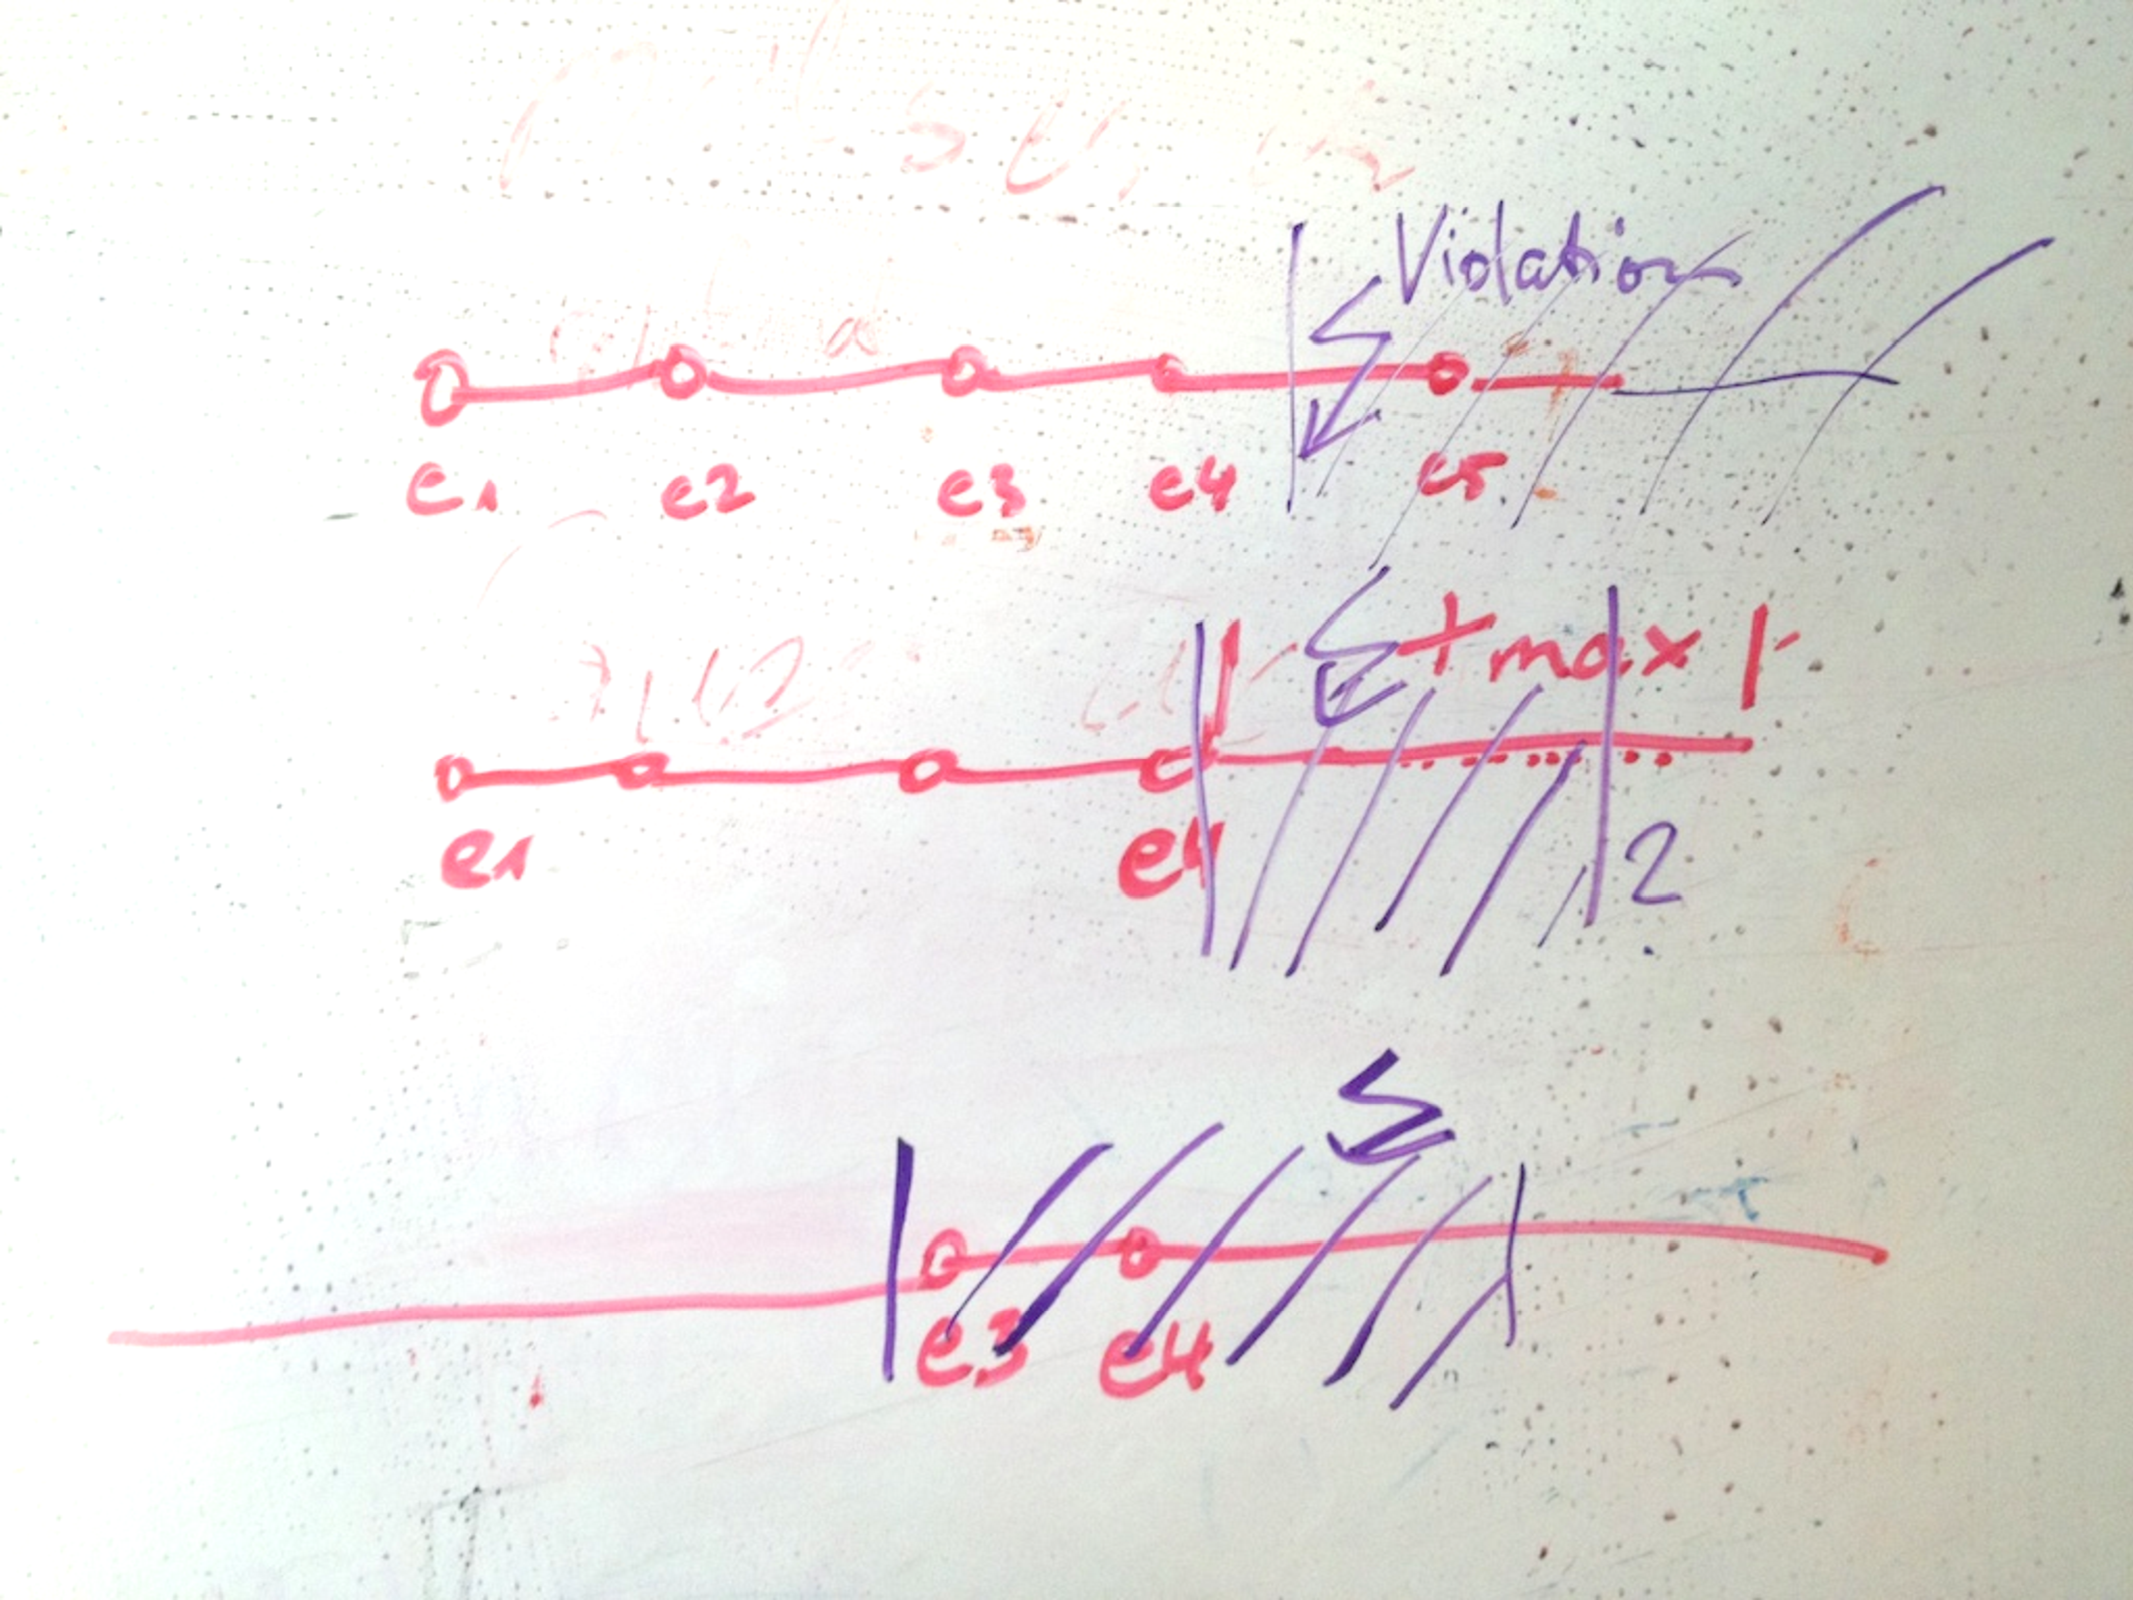
\includegraphics[width=3.25in]{../diagrams/approach/localizing}
    \caption[]{\label{fig:localizing} Localizing the minimal causal sequence for a failure in the 
    event stream}
\end{figure}



\subsection{Discussion}
Correspondence checking and \simulator{} serve to isolate the platform layer and
event sequence responsible for a given error. To identify the root cause of
the failure in the code, they can be complemented by classical debugging
techniques,\ie{} log messages and source code debugging. These are much more
effective when applied to investigate a specific event sequence. Once a
potential fix has been developed, it can be validated by repeating the
problematic replay. Fuzzing helps to validate whether there may be
related error events that the patch may have left open.

